\documentclass[10pt]{article}
\usepackage[margin=2cm]{geometry}
\usepackage{amsmath,amssymb,booktabs,graphicx,float,hyperref,xcolor}
\usepackage[font=small]{caption}
\setlength{\parindent}{0pt}
\setlength{\parskip}{3pt}
\newcommand{\E}{\mathbb{E}}
\newcommand{\Ch}{\widehat C}
\newcommand{\Vh}{\widehat V}
\newcommand{\taub}{\widehat\tau}

\title{MTH 9821 --- American Options: Policy Evaluation and Fitted Q-Learning}
\author{}
\date{}

\begin{document}
\maketitle
\vspace{-1.4cm}
\begin{center}
Team 9: Jaskaran Kalra, William McDonnell
\end{center}

Equation numbers (1)--(13) refer to the assignment. Every number below is produced by
\texttt{python src/run\_all.py \&\& python src/make\_tables.py} (see README).

%=====================================================================
\section*{1. The value function}

\textbf{(1) Fixed-policy value.} For a policy $a=(a_n)$ with $a_N\equiv1$,
\[
V^a_n(s,x)=\E\Big[\sum_{m=n}^{N}\beta^{m-n}\,x_m\,a_m(S_m)\,g(S_m)\;\Big|\;S_n=s,\;x_n=x\Big],
\qquad x_{m+1}=(x_m-a_m(S_m))^+ .
\]
By (4), $x_m a_m(S_m)=1$ only at the first exercise date $\ge n$ of an alive contract, so the sum is
the single discounted payoff. Separating the $m=n$ term and conditioning on $S_{n+1}$ (tower
property; $S$ is Markov and $x_{n+1}$ is a known function of $(s,x)$):
\[
V^a_n(s,x)=x\,a_n(s)\,g(s)+\beta\,\E\big[V^a_{n+1}\big(S_{n+1},(x-a_n(s))^+\big)\,\big|\,S_n=s\big],
\qquad V^a_N(s,x)=x\,g(s).
\]
\emph{Exercised option.} If $x=0$ then $(0-a_m)^+=0$, so $x_m=0$ for all $m\ge n$, every term of
the sum is zero and $V^a_n(s,0)=0$: exercise pays once and ends the contract.
\emph{Function vs.\ path.} $V^a_n(s,x)$ is a deterministic number for each $(s,x)$, a conditional
mean. Along one simulated path, the realized discounted cash flow
$\sum_m\beta^{m-n}x_m a_m g(S_m)$ is a random variable; its conditional mean is $V^a_n(s,x)$.
Policy evaluation averages these realized cash flows.

\textbf{(2) Bellman equation.} With $x=1$ the recursion gives two choices at date $n<N$.
Exercise ($a_n=1$) gives $g(s)+\beta\E[V_{n+1}(S_{n+1},0)]=g(s)$; continuing ($a_n=0$) gives
$\beta\E[V_{n+1}(S_{n+1},1)\mid S_n=s]$. Holding now and optimizing later defines
\begin{gather*}
C^*_n(s)=\beta\,\E\big[V^*_{n+1}(S_{n+1},1)\,\big|\,S_n=s\big],\qquad
V^*_n(s,1)=\max\{g(s),\,C^*_n(s)\}\quad(n<N),\\
V^*_N(s,1)=g(s),\qquad V^*_n(s,0)=0 .
\end{gather*}
\emph{Backward induction.} Claim: for any admissible policy $\pi$, possibly using the whole observed
history $\mathcal F_n$, the conditional expected remaining payoff of an alive contract is
$\le V^*_n(S_n,1)$, with equality for $a^*_n(s)=\mathbf 1\{g(s)\ge C^*_n(s)\}$. At $n=N$ settlement
is forced, so equality holds. Assume the claim at $n+1$. If $\pi$ exercises at $n$ it receives
$g(S_n)\le V^*_n(S_n,1)$. If it continues, its value is
$\beta\E[\E[\text{payoff}\mid\mathcal F_{n+1}]\mid\mathcal F_n]
\le\beta\E[V^*_{n+1}(S_{n+1},1)\mid\mathcal F_n]=C^*_n(S_n)$, where the last step uses the Markov
property: given $S_n$, $S_{n+1}$ is independent of the earlier history. So $\pi$ gets at most
$\max\{g,C^*_n\}=V^*_n$, and $a^*$, which picks the larger term at every date, attains it.
Hence no policy, history-dependent or not, beats $V^*_0(S_0,1)$.

\textbf{(3) Two-period check.} $q=(1.05-0.8)/(1.2-0.8)=0.625$. Terminal payoffs:
$S_{uu}=144\to0$, $S_{ud}=S_{du}=96\to4$, $S_{dd}=64\to36$.
\begin{itemize}\itemsep0pt
\item Up ($S_1=120$): $C_1=(0.625\cdot0+0.375\cdot4)/1.05=1.4286$, $g=0$ $\Rightarrow$ continue, $V_1=1.4286$.
\item Down ($S_1=80$): $C_1=(0.625\cdot4+0.375\cdot36)/1.05=15.2381<g=20$ $\Rightarrow$ exercise, $V_1=20$.
\item Inception: $C_0=(0.625\cdot1.4286+0.375\cdot20)/1.05=7.9932>g(100)=0$ $\Rightarrow$ continue, $V_0=7.9932$.
\end{itemize}
Up--down and down--up both end at 96, but on down--up the contract was exercised at $S_1=80$, so
$x_2=0$ and it receives nothing more; on up--down it is still alive ($x_2=1$) and pays 4 at $t_2$.
The alive state depends on the path, not only on the current price.

%=====================================================================
\section*{2. Longstaff--Schwartz}

\textbf{(1)--(2) Implementation} (\texttt{src/amop.py}, \texttt{train\_lsm}). Planned index
$\taub=N$ on every path. For $n=N-1,\dots,1$: form all responses (8), fit on in-the-money paths by
\texttt{lstsq}, clip by (6), then set $\taub=n$ where (7) holds. At $n=0$ the fitted value is
$\max\{\overline{Y_0},g(S_0)\}$ and the frozen decision uses the convention of (7). No fallback was
triggered in any of the twelve fits.

\textbf{(3) Questions.}
\emph{Cash flow, not fitted value.} $Y^{(i)}_n$ is the payoff actually realized on path $i$ by
following the already fitted future policy. It is one noisy draw whose conditional mean given
$S_n=s$ is the continuation value of that policy. Regression estimates this mean; no fitted value is
fed back into the responses, so regression error affects later fits only through the decisions.
\emph{Future information.} Responses are training labels. The regression projects them onto
functions of $S_n$ only, so the fitted rule uses the current price. In evaluation the decision must
be a stopping time; giving the policy future prices would be look-ahead (perfect foresight) and its
payoff would not be attainable.
\emph{Discount to date $n$.} Rule (7) compares the response with $g(S_n)$, paid at $t_n$. Both must be in
date-$n$ money. Discounting to date 0 would shrink the continuation estimate by $\beta^n$ and bias
the rule toward exercise.

%=====================================================================
\section*{3. Fitted Q-learning}

\textbf{(1)--(2) Implementation} (\texttt{train\_fq}). $\Vh_N=g$ on the training paths. For
$n=N-1,\dots,1$: targets (11) from the frozen $\Vh_{n+1}$, fit on all paths, clip by (6), then
$\Vh_n=\max\{g,\Ch_n\}$ by (12). At $n=0$: clipped average of (11) compared with $g(S_0)$. Actions
then come from (7), and the frozen policy is evaluated on the fresh evaluation set (Part 4).

\textbf{(3) Questions.}
\emph{From (9) to (11).} $Q^*_n(s,\text{continue})=\beta\E[V^*_{n+1}(S_{n+1},1)\mid S_n=s]=C^*_n(s)$.
Replace the unknown $V^*_{n+1}$ by the fitted $\Vh_{n+1}$ and the conditional expectation by a
least-squares regression on $\phi_d(S_n)$. Then $\beta\Vh_{n+1}(S^{(i)}_{n+1})$ is a sample with
conditional mean $\beta\E[\Vh_{n+1}(S_{n+1})\mid S_n=s]$, which is (11).
\emph{Contrast with (8).} In (11) only one transition $S_{n+1}$ is realized and the rest is
\emph{estimated} ($\Vh_{n+1}$). Its variance is low, but regression error and the upward bias of
the $\max$ in (12) carry backward through all dates. In (8) the whole future cash flow is
\emph{realized} and only the decisions are estimated, so the variance is higher but no fitted value
is propagated.
\emph{Out of the money.} With $s>K$ the stock can still fall below $K$ before maturity, so
$C^*_n(s)>0$. In this recursion $\Vh_n=\Ch_n$ on such states, and those values become targets at
date $n-1$ for every path that is out of the money at $n$. A fit on in-the-money states only would
supply these values by extrapolating the polynomial outside its data (clipped to $0$ or $K$, or
badly wrong), and the error would enter all earlier targets. LSM does not have this problem: out of
the money the decision is always ``continue'', and its responses are realized cash flows.

%=====================================================================
\section*{4. Comparison of frozen policies}

Training seeds 17, 29, 43 (20,000 paths each, shared by both methods and degrees); one evaluation
set, seed 20261008, 100,000 paths, used for every policy and never for tuning. Benchmark: finest
tree value $6.07861$ (change from previous refinement $0.00003$).

\textbf{(1) Checks and results.}
\emph{Evaluator:} enumerating the four two-period paths with weights $q^2,q(1-q),(1-q)q,(1-q)^2$ and
discount $1/1.05$ gives $7.993197$, equal to $V_0$ above (exercise dates: up--up and up--down at
$t_2$, down--up and down--down at $t_1$).
\emph{European:} $\beta^N g(S_N)$ on the evaluation set gives $5.5876$ (SE $0.0274$) vs.\ Black--Scholes
$5.5735$; $z=0.51$.
\emph{Reference:} an independent CRR tree (2500 steps, exercise every 50 steps) gives $6.0783717$,
equal to the supplied 2500-step value.

\begin{table}[H]\centering\small
\begin{tabular}{rllrrrcrr}
\toprule
seed & method & $d$ & fitted $V_0$ & policy value & SE & 95\% CI & train (s) & eval (s) \\
\midrule
17 & LSM & 2 & 5.9756 & 6.0589 & 0.0227 & [6.0144, 6.1033] & 0.18 & 0.38 \\
17 & FQ & 2 & 7.8539 & 5.8516 & 0.0264 & [5.7998, 5.9035] & 0.15 & 0.38 \\
17 & LSM & 4 & 5.9903 & 6.0780 & 0.0226 & [6.0337, 6.1223] & 0.22 & 0.34 \\
17 & FQ & 4 & 6.9007 & 6.0191 & 0.0243 & [5.9716, 6.0667] & 0.15 & 0.38 \\
\midrule
29 & LSM & 2 & 6.0806 & 6.0518 & 0.0224 & [6.0079, 6.0958] & 0.19 & 0.48 \\
29 & FQ & 2 & 7.9505 & 5.8505 & 0.0265 & [5.7985, 5.9025] & 0.18 & 0.43 \\
29 & LSM & 4 & 6.1011 & 6.0699 & 0.0225 & [6.0259, 6.1139] & 0.22 & 0.44 \\
29 & FQ & 4 & 6.9897 & 6.0050 & 0.0246 & [5.9568, 6.0532] & 0.23 & 0.48 \\
\midrule
43 & LSM & 2 & 6.0950 & 6.0560 & 0.0229 & [6.0111, 6.1010] & 0.22 & 0.39 \\
43 & FQ & 2 & 7.9321 & 5.8494 & 0.0265 & [5.7974, 5.9014] & 0.21 & 0.49 \\
43 & LSM & 4 & 6.1032 & 6.0774 & 0.0227 & [6.0329, 6.1219] & 0.31 & 0.55 \\
43 & FQ & 4 & 7.0090 & 5.9778 & 0.0248 & [5.9291, 6.0265] & 0.23 & 0.41 \\
\bottomrule
\end{tabular}

\caption{Twelve frozen policies. Policy value, SE and CI from (13) on the evaluation set. Times
exclude path simulation ($\approx$0.04\,s per training set, 0.21\,s for the evaluation set; see
\texttt{results.csv}).}
\end{table}
\vspace{-2mm}
\emph{Discrepancies.} (i) FQ fitted values (6.90--7.95) exceed their policy values by 0.9--2.1,
roughly 35--80 SE: this is not Monte Carlo error. Each date's fitted value inherits the regression
error of all later dates, and the $\max$ in (12) turns that error into an upward bias. A degree-2
polynomial fitted on all paths also places $\Ch_n$ above $g$ in the region where exercise is
optimal, so the policy exercises too late. Raising the degree to 4 lowers the fitted value by about
0.95 and raises the policy value by 0.13--0.17, consistent with approximation error.
(ii) LSM fitted values differ from policy values by $-0.08$ to $+0.04$. They are averages over only
20,000 training paths (SE $\approx 0.05$), so these gaps are within about 1.6 training SE.
(iii) All twelve policy values lie below the benchmark; LSM $d=4$ is within 0.009 of it for every seed.

\textbf{(2) Paired comparisons} (FQ $-$ LSM on common evaluation paths, (13) on the differences).

\begin{table}[H]\centering\small
\begin{tabular}{rlrrc}
\toprule
seed & $d$ & FQ $-$ LSM & SE & 95\% CI \\
\midrule
17 & 2 & -0.2072 & 0.0149 & [-0.2365, -0.1779] \\
17 & 4 & -0.0589 & 0.0094 & [-0.0773, -0.0404] \\
29 & 2 & -0.2013 & 0.0154 & [-0.2315, -0.1711] \\
29 & 4 & -0.0649 & 0.0106 & [-0.0856, -0.0442] \\
43 & 2 & -0.2066 & 0.0147 & [-0.2355, -0.1777] \\
43 & 4 & -0.0996 & 0.0109 & [-0.1210, -0.0782] \\
\bottomrule
\end{tabular}

\caption{FQ $-$ LSM by seed and degree (\texttt{paired.csv}).}
\end{table}
\vspace{-2mm}
All six FQ $-$ LSM intervals lie below zero: LSM gives the better policy for every seed and degree.
The gap is about $-0.20$ at $d=2$ and $-0.06$ to $-0.10$ at $d=4$. Pairing removes the common path
noise: the paired SE (0.009--0.015) is well below the $\approx0.034$ an unpaired difference would have.
Degree 4 narrows the FQ $-$ LSM gap for every seed. From Table 1, degree 4 raises the policy value for both
methods: LSM from $6.052$--$6.059$ to $6.070$--$6.078$, FQ from $5.849$--$5.852$ to $5.978$--$6.019$. Across seeds, the LSM $d=4$ policy values range over $6.070$--$6.078$ and FQ $d=4$
over $5.978$--$6.019$, so FQ is also more sensitive to the training sample. Three seeds are too few to
estimate this spread precisely, and the twelve prices are not pooled.

\textbf{(3) Decisions at $n=25$, seed 17.}
\begin{figure}[H]\centering
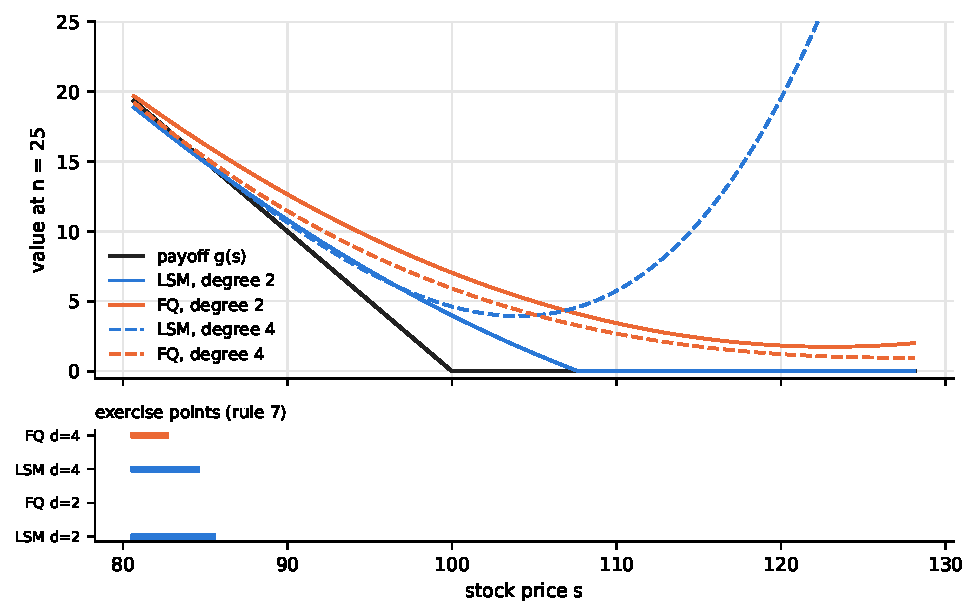
\includegraphics[width=0.72\textwidth]{../figures/n25_decisions.pdf}
\vspace{-2mm}
\caption{Clipped continuation $\Ch_{25}$ and $g$ on 200 spots between the 5th and 95th percentiles
of the date-25 training spots (80.7--128.1). Bottom: grid points where (7) exercises.}
\end{figure}
\vspace{-3mm}
The exercise regions were computed point by point. On this grid each is a single interval:
LSM $d=2$ exercises for $s\le85.4$, LSM $d=4$ for $s\le84.5$, FQ $d=4$ for $s\le82.6$, and
FQ $d=2$ never exercises ($\Ch_{25}>g$ everywhere). The LSM $d=4$ curve rises sharply out of the
money because it is fitted on in-the-money paths only; there $g=0$, so the policy continues anyway.
\emph{More flexible fit:} yes, the independently evaluated price improves with degree 4 for both
methods (Table 1), a lot for FQ and slightly for LSM.
\emph{Small price impact near a crossing:} where $g(s)\approx C^*_n(s)$, choosing the wrong action
loses only $|g(s)-C^*_n(s)|\approx0$. A small shift of the boundary therefore costs little: the LSM
$d=2$ and $d=4$ boundaries differ by about 1 in $s$, yet their prices differ by only about 0.02.

\textbf{(4) Interpretation.} Conditional on the training data $D$, a frozen policy is a fixed rule
using only $(n,S_n)$, and the evaluation paths are independent of $D$. It is therefore admissible,
and by Part 1(2)
$\E[H\mid D]=V^{\hat a}_0(S_0,1)\le V^*_0(S_0,1)\approx6.0786$.
\emph{Test means} estimate $\E[H\mid D]$ with error of order one SE ($\approx0.023$), so a policy close
to optimal can produce a sample mean above $V^*_0$ by chance.
\emph{Fitted values} are not payoffs of an admissible policy. LSM's is an in-sample average on the
same paths used to choose the decisions (optimistic, plus training noise). FQ's is built from fitted
values with an upward $\max$ bias and basis error. Neither has to lie below $V^*_0$, and FQ's do not.
\emph{What the SEs measure:} only evaluation Monte Carlo noise for a fixed policy. They omit:
training-sample variation (a different seed gives a different policy; compare the seed spread),
approximation error from the polynomial basis and degree, and reference error (finite tree; the last
refinement change $0.00003$ is an empirical check, not a bound).

%=====================================================================
\section*{Use of AI assistance}
We used Claude (Anthropic) as our AI assistant for derivation checks,
code drafting and debugging, and report and slide drafting. We checked the work independently of it:
the two-period model by hand and by path enumeration through the shared evaluator; the European
price against Black--Scholes; the reference with our own CRR tree; the vectorized evaluator against
a path-by-path loop version (maximum difference $4\times10^{-15}$); and the effect of the degree on both fitted and policy values. Both partners reviewed the derivations
and the code and can explain them.

\end{document}
